\chapter*{Introduction}\addcontentsline{toc}{chapter}{Introduction}
Amidst the countless stars and galaxies we observe in the Universe lie 
undetected structures of dark matter, orders of magnitude larger than 
the luminous objects they engulf. These vast invisible structures began 
in the very early Universe, as quantum fluctuations in the aftermath of 
the Big Bang. 
%These vast invisible structures began as quantum fluctuations in the beginning of the Universe in the aftermath of the Big Bang. 
During the subsequent period of inflation (\todo{cite?}), these primordial fluctations 
were amplified by the accelerated expansion of the Universe and then 
propagated through gravitational instability for billions of years. 

Despite constituting most of the matter in the Universe, dark matter 
has yet to be directly observed. In fact, it can only be studied through 
its gravitational interactions with luminous baryons — the matter that 
constitutes stars, galaxies, and celestial objects that emit light. 
In a way, the galaxies we observe in the cosmic volumes probed by our 
telescopes act as illuminated beacons tracing the vast dark matter 
terrains of the Universe.

Over the past decade, spectroscopic redshift surveys like the 
Baryon Oscillation Spectroscopic Survey (BOSS\todo{cite}) have 
exploited these galactic beacons to map out the cosmic structure
of the Universe. Precise measurements of distance and growth 
of large-scale structure (LSS) from these surveys, provide tests 
of cosmological models that desribe the content, geometry and history 
of the Universe. \todo{By analyzing measurements of LSS,}


Through these galaxies, we can explore the properties of the underlying dark matter
and the growth of their structure. Measurements that quantify these properties allow us to make
precise calculations of cosmological parameters, which quantify the content, geometry, and
expansion history of the Universe. Ultimately the constraints we measure on these parameters,
enlighten us on the properties of dark energy, which remains one of the most crucial unsolved
questions in cosmology. Certainly these precise cosmological measurements require a profound
understanding of the formation and evolution of galaxies. Unfortunately there is no clear
narrative of galaxy formation and evolution due to the complex, non-linear, and stochastic nature
of the physical processes that govern them.

In fact, galaxy formation and evolution remain another central unsolved questions in
astrophysics and cosmology. However, since galaxies are enveloped in the massive gravitational
wells of their host dark matter structures, the underlying dark matter of galaxies undoubtedly
plays a crucial role in their formation and evolution. Therefore, with its implications on the most
crucial questions in both cosmology and our understanding of galaxies, the interactions between
galaxies and their host dark matter environments pose some of the most impactful questions,
questions that I seek to answer in my dissertation. 


%\section{$\Lambda$CDM cosmology}
\section{Large Scale Structure} \label{sec:lss}
From the early Universe, primordial quantum fluctuations grow into the 
large-scale structures of the Universe we observe today through the different
epochs of cosmic history and by gravitational instability. In this section, I briefly 
describe the simplified ({\em linear}) theory of this evolution and explain core 
concepts of LSS cosmology using galaxies. Lets begin by defining the matter 
overdensity field (or density fluctuation) at comoving position ${\bf r}$: 
\beq \label{eq:delta}
\delta({\bf r}) = \frac{\rho({\bf r}) - \bar{\rho}}{\bar{\rho}}, 
\eeq
where $\rho({\bf r})$ and $\bar{\rho}$ are the density field and mean 
density respectively. In Fourier space ($k$-space), Eq.~\ref{eq:delta} can 
be Fourier transformed, 
\beq
\delta({\bf k}) = \int \frac{{\rm d^3}{\bf r}}{(2\pi)^3} e^{-i{\bf k}\dot{\bf r}}\;\delta({\bf r}).
\eeq
For describing the evolution of the overdensity field, Fourier space is generally 
favored over configuration space because, as derived later in the section,
the Fourier modes of $\delta$ evolve independently in linear theory -- 
\emph{i.e.} on large scales.

The information in the overdensity field is often quantified using its 
$N$-point statistics (\todo{cite Peebles bernardeua}). In fact, the two-point
statistic is one of commonly used tool in large scale structure studies.
This two-point statistic (also referred to as the correlation function) is
defined as, 
\beq
\xi(r) = <\delta({\bf x})\delta({\bf x} +  {\bf r})>
\eeq
and in Fourier space as,
\beq
<\delta({\bf k})\delta({\bf k'})> = (2\pi)^3 P(k) \delta^{D}({\bf k}+{\bf k'}).
\eeq
$\delta^{D}$ is the Dirac delta function and $P(k)$ is the {\em powerspectrum}, 
the Fourier transform of $\xi$. In principle, $\xi$ and $P(k)$ contain the same 
information. In practice, however, analyzing $\xi$ versus $P(k)$ carry different 
caveats (\todo{cite FKP}). Throughout this section, and also the dissertation, 
I will mainly focus on the powerspectrum. 

The evolution of the dark matter overdensity field can be derived (on 
sub-horizon scales) as follows. For pressureless dark matter, the equation of motion
can be derived from the continuity, Euler, and Poisson equations
\beqa 
\frac{\partial \rho}{\partial t} + \nabla \dot \rho {\bf u} = 0  \\ 
\frac{\partial {\bf u}}{\partial t} + ({\bf u} \dot \nabla) \dot {\bf u} - \nabla\Phi = 0 \\ 
\nabla^2\Phi - 4 \pi G \rho = 0 
\eeqa
to 
\beq \label{eq:meszaros}
\frac{\partial^2 \delta}{\partial t^2} + 2 \frac{\dot{a}}{a} \frac{\partial \delta}{\partial t} - 4 \pi G \bar{\rho} \delta = 0.
\eeq
${\bf u}$ is the velocity field, $\Phi$ is the gravitational potential, and $a$ 
is the scale factor. For a detailed derivation I refer readers to \todo{cite Peebles 
or Dodelson}. Eq.~\ref{eq:meszaros} a second order differential equation, therefore,
the solution can be written as 
\beq 
\delta({\bf r}, t) = D^{(+)}(t) A({\bf r}) + D^{(-)}(t) B({\bf r}).
\eeq
The density flucation has two components: a growing mode $D^{(+)}$ and a decaying 
mode $D^{(-)}$. The decaying mode decreases with time and its contribution becomes negligible
leaving only the growing mode in the late Universe. Now in order to quantify
the evolution of the growing mode $D^{(+)}$, one commonly used quantity is the 
``growth rate of structure'': 
\beq \label{eq:f_growth}
f = \frac{ d {\rm ln}\;D^{(+)}}{d {\rm ln}\;a}. 
\eeq
This growth rate of structure is a key quantity in LSS cosmology for testing different 
cosmological models and theories of gravity. $f$ will be discussed further in Section~\ref{sec:rsd}.

From the early Universe the density fluctuations evolve through different epochs in 
cosmic history: inflation, radiation-dominated, and matter-dominated eras. Each of 
these periods leave an imprint on the evolution of $\delta$. Fig.~\ref{fig:lifo}, 
marks the different eras in the early Universe and plots how the physical scale of 
the Universe, represented by the Hubble radius, evolves with $a$. 

During inflation, the Hubble radius remains constant. Afterwards the Universe 
becomes radiation dominated. Based on the Friedmann equations the Hubble radius 
during the radiation dominated era is approximately $\propto a^{2}$. The Universe then 
becomes matter dominated and the Hubble radius is approximately $\propto a^{3/2}$. 
Meanwhile, the physical scale of perturbations is 
$\lambda_{phys} = \lambda_{comov}\ a(t) \propto a(t)$. As Fig.~\ref{fig:lifo} 
illustrates, perturbations exit the Hubble radius during inflation then 
reenter the Hubble radius later on. Depending on the physical scale of the 
perturbation, it can enter either during the radiation dominated  
(smaller scale) or matter dominated (larger scale) era. 


The physical scale of perturbations that enter the horizon at the time of 
matter-radiation equality ($a(t) = a_{eq}$), $\lambda_{eq}$ is $\sim 500 h^{-1}Mpc$.
The perturbations that enter before the matter-radiation equality during 
the radiation dominated era, have physical scales $\lambda_{phys} < \lambda_{eq}$. 
These smaller scale perturbations, todo{explain the supression} 
On the other side, the larger scale perturbations with $\lambda_{phys} > \lambda_{eq}$
enter after matter-radiation equality during the matter dominated epoch. These 
perturbations do {\em not} experience the suppression of growth of the radiation 
dominated era. Therefore, as the overdensity field goes through these epochs, its 
growth on small scale is suppressed by a factor of $\sim k^4$.  


In practice, this scale dependent evolution of the density fluctuation is 
quantified through the ``transfer function'' $T(k)$ (\todo{cite all the transfer function papers}). After inflation the 
powerspectrum of the density fluctation can be summarized by: 
\beq
P_{inf}(k) \propto k^{n_s}
\eeq
where $n_s \sim 1$ \todo{cite inflation papers: Harrison (1970), Zel’dovich (1972) and Peebles Yu (1970) Komatsu et al. 2011}. Then powerspectrum of the density 
fluctuation in the late Universe can be expressed as 
\beq
P(k) \propto k^{n_s} T^2(k) D^2(k). 
\eeq
$D(k) \equiv D^(+)$ from earlier this section. 

\begin{figure*}
\begin{center}
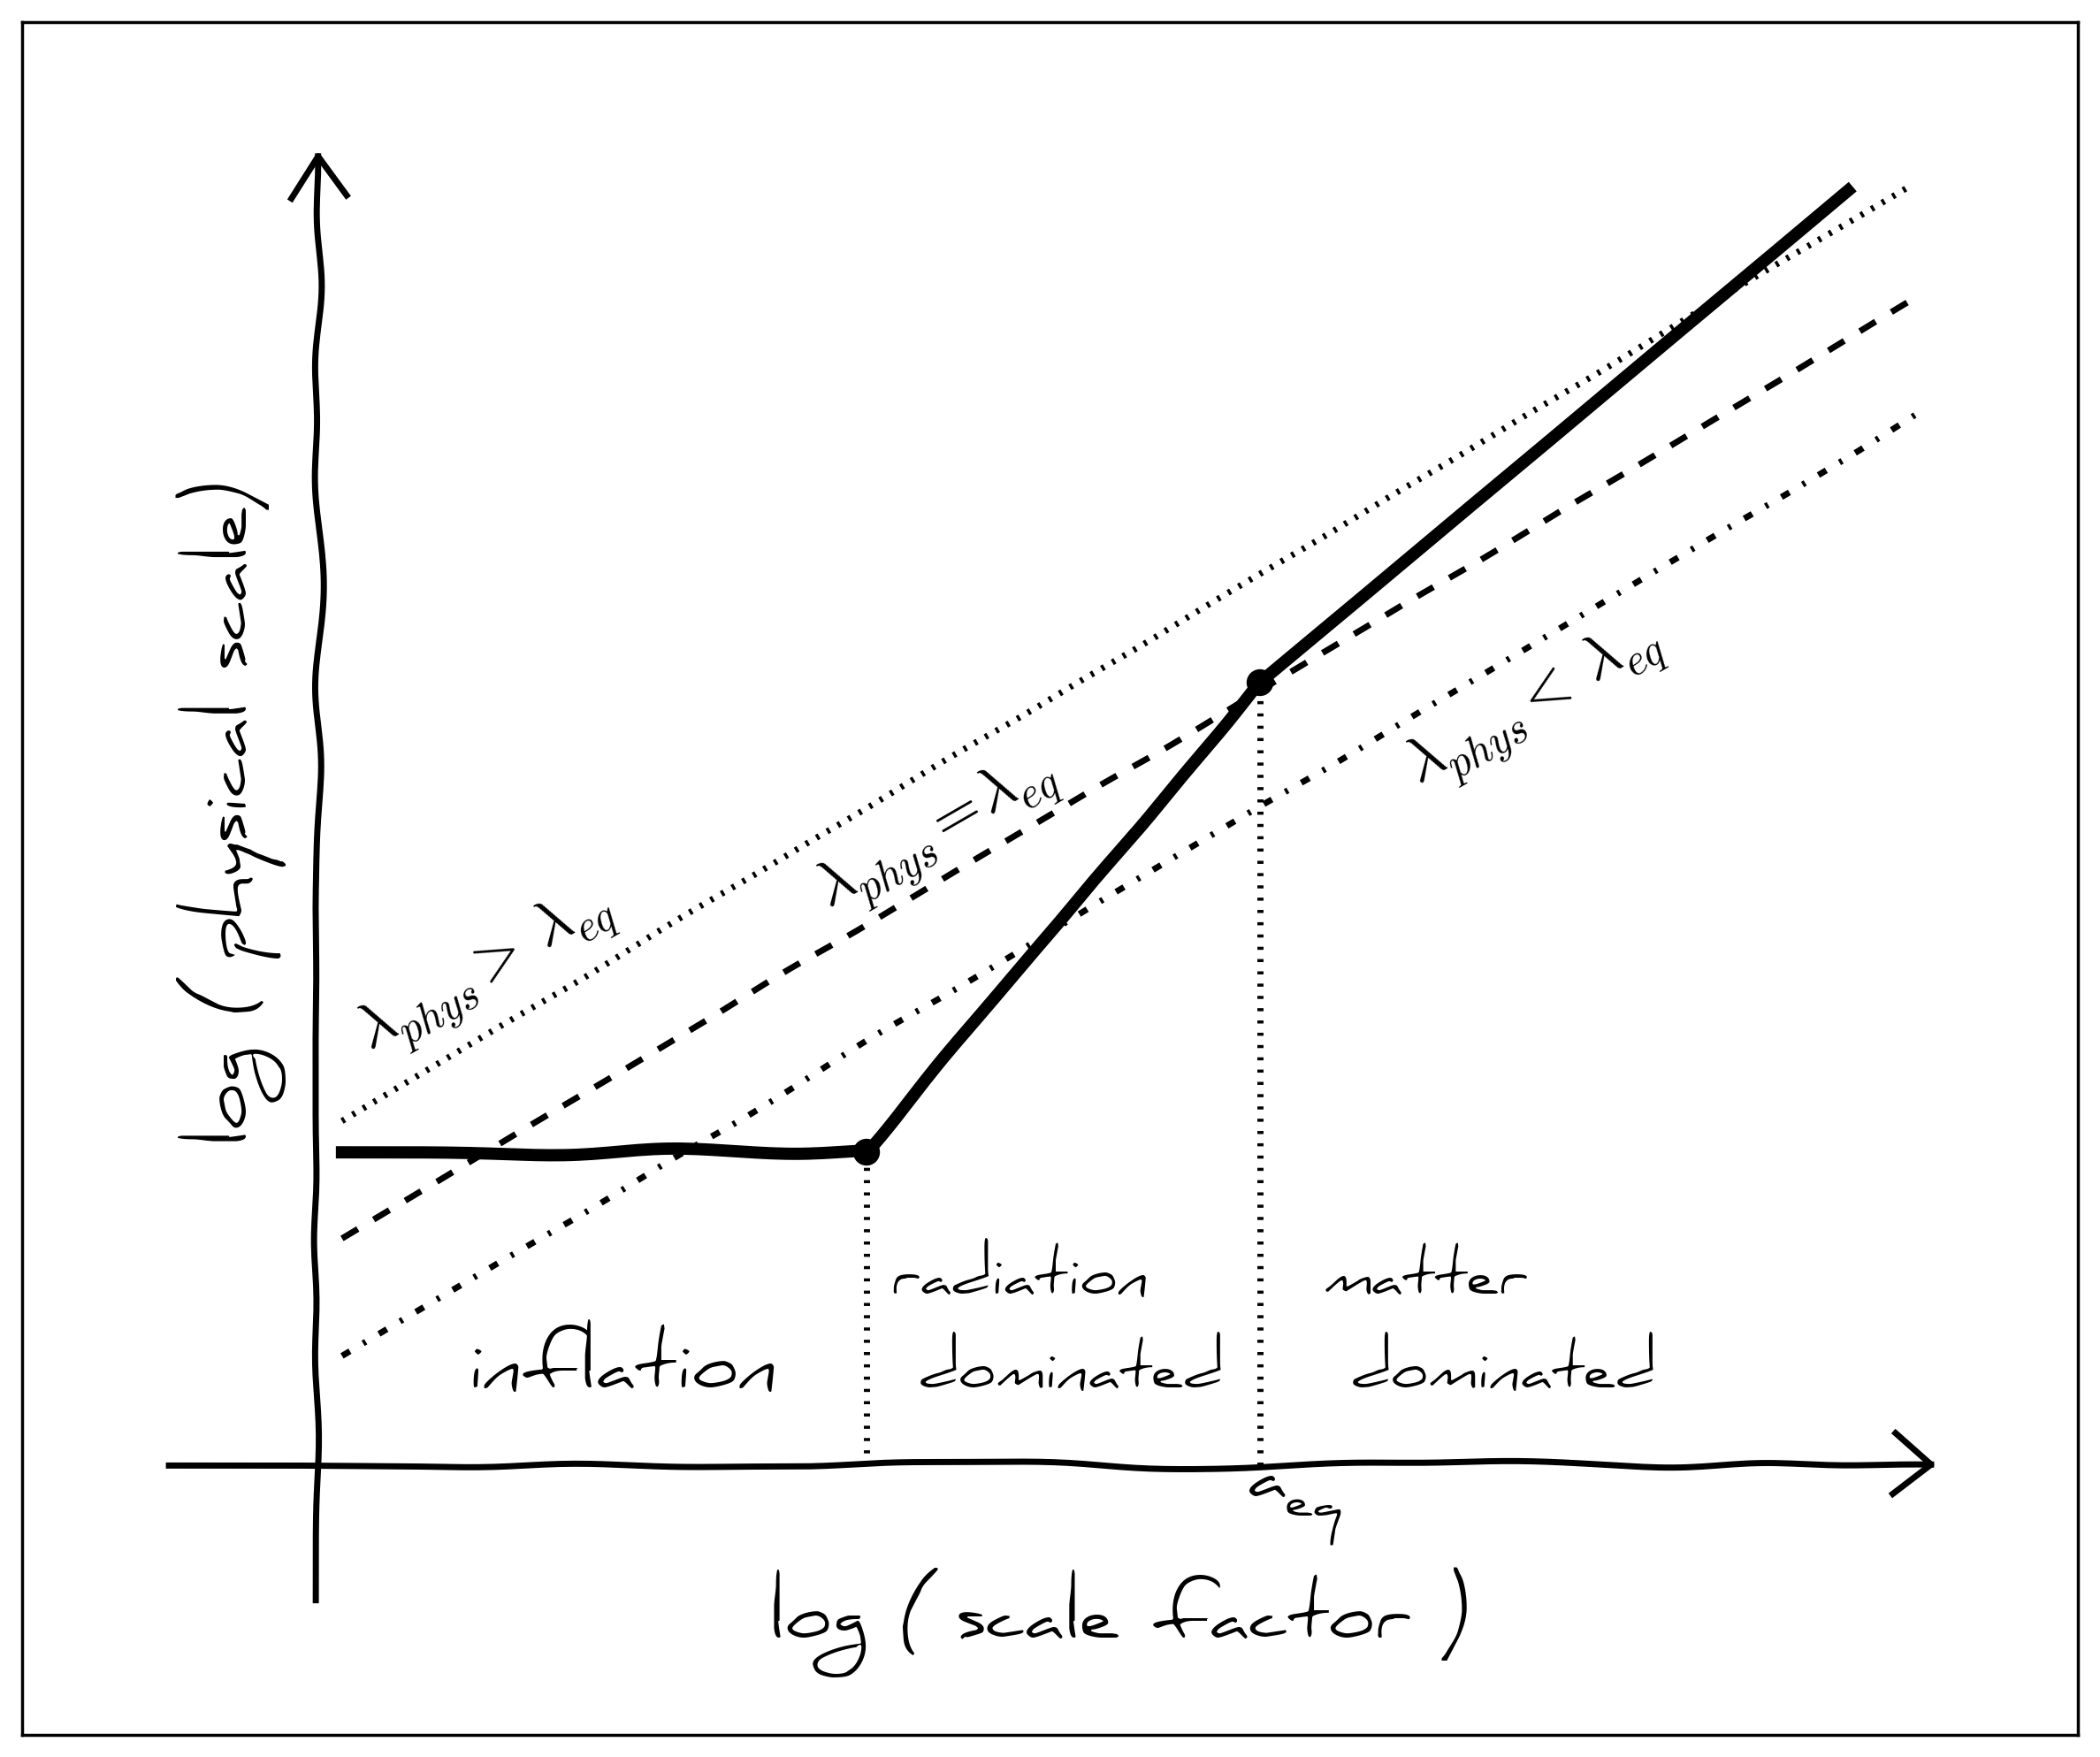
\includegraphics[width=\textwidth]{figs/lifo.png}
\caption{Schematic diagram that illustrates the evolution of the Hubble radius
(Above) The evolution of the Hubble radius (solid line) during inflation (flat), radiation
domination, and matter domination (note inflection). Dashed, dotted, and dot-dashed
lines show the physical length of three constant comoving scales. The scale corresponding
to the current Hubble radius cH−1
0 first “left the horizon” about 60 e-folds before the end
of inflation (open circle).
} \label{fig:lifo}
\end{center}
\end{figure*}

\todo{paragraph about how because D and T depend on cosmological parameters 
    so powerspectrum measurements of the matter density fluctuation can be 
    used a tests of the cosmological models.
}
So powerspectrum measurements of the matter density fluctuations can be compared
to predictions of various cosmological models in order to produce constraints 
on cosmological parameters, better understand dark energy, and test theories of 
gravity. Unfortunately, most of the matter in the Universe is in the form of dark 
matter and does not interact with radiation. 

Observers cannot measure the spatial statistics (or clustering) of dark matter 
directly. Instead, we measure the clustering of galaxies and quasars, which trace
the underlying matter distribution. The smoothed galaxy/quasar density field is 
approximated by a local function of the matter density field
\beq
\delta_g({\bf r}) = F( \delta({\bf r} ). 
\eeq
This function can then be expanded Taylor series,
\beq
\delta_g({\bf r}) = \sum\limits_{k=0}^{\infty} \frac{b_k}{k!} \delta^k. 
\eeq
$b_1$ is referred to as the linear bias factor and $b_0$ is chosen so that
$<\delta_g> = 0$. To linear order, 
\beq
P_g(k) = b_1^2 P(k). 
\eeq
The primary subpopulation of galaxies used so far for LSS studies are luminous 
red galaxies (\todo{Eistenstien apper}). These galaxies have $b_1 > 1$, which 
means they are {\em biased} tracers of the matter distribution (\todo{cite Zehavi 2005, Sheldon 2009, Gastanage 2009}). 
This bias is caused by the fact that luminous galaxies reside in larger potential 
wells, which have stronger clustering properties than than less massive ones (\todo{manera 2010}). 

Based on the simplified derivation of this section, once we have the spatial 
distribution of galaxies or quasars we can derive the clustering of the matter
distribution and then infer cosmological constraints. In practice, however, a
number of factors complicate this procedure. One key complication is redshift-space
distortions, which will be discussed in the following section.

\section{Redshift-Space Distortions} \label{sec:rsd}
Spectroscopic redshifts surveys, such as 2dFGRS, SDSS, and BOSS, have mapped out
millions of distant galaxies. Current surveys such as Extended Baryon Oscillation 
Spectroscopic Survey (eBOSS; \citealt{Dawson:2015aa}), and future surveys such as 
the Dark Energy Survey Instrument (DESI; \citealt{Schlegel:2011aa, Morales:2012aa, Makarem:2014aa}) 
and the Subaru Prime Focus Spectrograph (PFS; \citealt{Takada:2014aa}), will 
continue to map out millions more. These surveys dominate LSS studies and have/will 
been critical for inferring precise cosmological constraints. As their name suggest, 
however, these {\em redshift} surveys do not directly measure the position of 
galaxies, but rather the angular positions (right ascension and declination) and
redshift of galaxies. 

Redshifts from spectroscopic surveys observe the combination of recession 
velocities due to the expansion of the Universe and the peculiar velocities of the galaxies 
\beq
z_{obv} = z_{true} +  \frac{v_{pec}}{c}.
\eeq 
The comoving positions derived from the angular positions and redshifts are then
in {\em redshift-space} and ``distorted'' compared to real-space comoving positions:
\beq
{\bf s} = {\bf x} +  \frac{{\bf v}_{pec} \cdot \hat{n}}{H_0}.
\eeq 
$\hat{n}$ is the unit vector along the line-of-sight. Thankfully, all hope is not 
lost. The peculiar velocities of galaxies should be directly related to the total 
matter distribution, since galaxies can be thought of as test particles in a 
gravitational field. 

\todo{Kaiser 87} derives an approximation for the distortion caused by the coherent 
infall of galaxies onto over dense regions in redshift space. This redshift-space 
distortion (RSD), often referred to as the Kaiser effect, causes overdense regions
to appear squashed along the line of sight in redshift space. Galaxies around an
overdense region closest to the observer (us) are moving towards the center of the 
overdense region, so they appear in redshift-space to be farther away. Galaxies 
on the other side of the overdense region are moving towards it and the observer, 
so they appear closer to us. 

More precisely, the relation between the overdensity field in redshift-space can be 
derived from the continuity equation and the distant observer approximation, 
\beq
\delta^{(s)}({\bf k}) = (1 + f \mu^2) \delta({\bf k}).
\eeq
$f$ here is the growth rate of structure from Eq.~\ref{eq:f_growth} and 
$\mu = {\bf k} \cdot \hat{n} / k$, cosine of the angle between $k$ and 
the line of sight. 

The Kaiser effect can be combined with the galaxy bias model from 
Section~\ref{sec:lss}, in order to express the galaxy overdensity field in 
redshift-space:
\beq
\delta_g^{(s)}({\bf k}) = (b + f \mu^2) \delta({\bf k}).
\eeq
The redshift-space powerspectrum of the galaxy overdensity field can then be
written as 
\beq
P_g^{(s)}(k, \mu) = (b + f \mu^2)^2 P(k).
\eeq
On large scales and with small overdensities, the effect of redshift-space 
distoritons is well described by the Kaiser effect. On small scales with large
overdensities things get a little more complicated. 

The random peculiar velocities of galaxies in gravitationally bound structures 
such as clusters cause their position in redshift-space along the line-of-sight 
to be smeared out to larger scales.  This effect can easily be identified by 
eye in galaxy redshift maps. The elongations of the galaxy positions along the 
line-of-sight look like fingers pointing towards the observer. Hence this 
redshift-space distorion is called the ``fingers-of-god''. Its impact on the 
powerspectrum, is typically quantified using an overall exponential factor such as 
\beq
P_g^{(s)}(k, \mu) \approx e^{-f^2 \sigma_v^2 \mu^2 k^2} (b + f \mu^2)^2 P(k).
\eeq
$\sigma_v$ is a paramter quantifying the strength of the effect and is usually
left as a free parameter. 

The relations that quantify the impact of RSDs reveal another means of measuring 
$f$. Consider the Legendre expansion of $P_g^{(s)}(k, \mu)$, 
\beq
P_g^{(s)}(k, \mu) = \sum\limits_{\ell=0, 2, 4 ...} \mathcal{L}_\ell(\mu) P_g^\ell(k). 
\eeq
Each of the powerspectrum ``multipoles'' of this expansion can be written as 
\beq
P_g^{\ell}(k) = \frac{2 \ell + 1}{2} \int\limits_{-1}^{1} {\rm d}\mu \; P_g^{(s)}(k, \mu) \mathcal{L}_\ell(\mu).
\eeq
The powerspectrum multipoles for $\ell= 0$ (monopole) and $2$ (quadrupole), neglecting 
the figers-of-god which does not significantly impact larger scales, are
\beqa
P_g^0 (k) = (b_1^2 + \frac{2}{3} f b_1 + \frac{1}{5}f^2) P(k) \\
P_g^2 (k) = (\frac{4}{3} f b_1 + \frac{4}{7} f^2) P(k). 
\eeqa
Their ratio 
\beq
\frac{P_g^2}{P_g^0} = \frac{\frac{4}{3} f b_1 + \frac{4}{7} f^2}{b_1^2 + \frac{2}{3} f b_1 + \frac{1}{5}f^2},
\eeq
illustrates how the distortions caused by RSDs allow us to extract information of 
$f$ through measurements of the redshift-space galaxy powerspectrum!  

\section{Weighting Neutrinos with Galaxies} \label{sec:mneut}
Beyond providing a way to infer the growth rate of structure, which 
can be used to test GR and modified gravity scenarios, galaxy clustering
also provides a unique window to probe fundamental physics beyond the 
standard model. 
In the derivations of Sections~\ref{sec:lss} and~\ref{sec:rsd} we focused 
on how the density fluctuations of dark matter evolves. Because dark matter 
consistutes majority of the matter in the Universe, this is an excellent 
approximation. However, it negelects some of the more detailed imprints on 
large-scale structure from other matter components-- \emph{i.e.} neutrinos. 
Oscillation and detection experiments have (\emph{very} Nobel Prize in Physics 2015) 
convincingly confirmed {\em not} massless (\todo{Beringer et al. 2012,Lesgourges, 2012, 2013})

In the very early Universe, neutrinos are relativistic and coupled to the 
primordial plamsa. Later they decouple from the plasma, while they are still 
ultra-relativistic and redshift. While they are relativistic, they do not 
contribute to the energy density of matter but instead radiation. Then during 
matter domination, neutrinos eventually become non-relativistic. At this point, 
neutrinos contribute to the matter energy density and act as ``warm/hot'' 
dark matter.

Neutrinos after they decouple from the primoridal plasma constitutes a 
collisionless fluid, where the individual particles free-stream with 
characteristic velocities defined by their thermal velocity. While 
neutrinos are relativistic, their free-streaming scale is simply 
equal to the Hubble radius. But when they become non-relativistic, 
their can be expressed as
\beq
v_{\rm th} \approx 158 (1 + z) \left(\frac{1 {\rm eV}}{m} \right) \; \; {\rm km \; s^{-1}}
\eeq
and the free-streaming scale can be derived in an analogous way as
Jean's length
\beq
\lambda_{\rm FS} = 2 \pi \sqrt{\frac{2}{3}} \left( \frac{v_{\rm th}}{H} \right)
\eeq
or 
\beq \label{eq:kfs}
k_{\rm FS} = \frac{2\pi a}{\lambda_{\rm FS}} \approx  0.82 \frac{\sqrt{\Omega_\Lambda + \Omega_m(1+z)^3}}{(1+z)^2} \left(\frac{m_\nu}{1\;{\rm eV}} \right).
\eeq
$\Omega_\Lambda$ and $\Omega_m$ are the current cosmological constant and matter 
density fractions, respectively.

Neutrinos leave two main imprints on LSS. In the early Universe they contribute
to the radiation energy density. After they become non-relativistic in matter
domiation, they contribute to the matter energy density. As described in 
Section~\ref{sec:lss}, matter-radiation equality marks the turning point in 
suppression of growth of structure, quantified by $T(k)$. The transition of 
neutrinos from radiation to matter impacts $a_{eq}$ and thus shifts the turning 
point of the cold dark matter (CDM) only powerspectrum. 
Even after becoming non-relativistic, neutrinos do not contribute to the
clustering of matter on scale smaller than the free-streaming scale, 
$k_{\rm FS}$ (Eq.~\ref{eq:kfs}). The impact of this scale dependent 
suppression of clustering, can be analytically estimated for the powerspectrum: 
\beq
\frac{\Delta P}{P} = \frac{P^{f_\nu \neq 0} - P^{f_\nu = 0}}{P^{f_\nu = 0}} \approx - 8 f_\nu \;\;\;\; {\rm for}\;\; k \gg k_{\rm FS}.
\eeq
$f_\nu = \Omega_\nu / \Omega_m$.

The total mass of neutrinos (\mneut) dictate the strength of these imprints. 
The broadband shape of the powerspectrum offers a unique opportunity to measure
the extent of these imprints and constrain \mneut. The same tools that we 
use for analyzing RSDs and measuring the growth rate of structure can be used 
to measure \mneut from observations of galaxy surveys.
Based on their forecasts (DESI; \todo{cite}), the next galaxy surveys have the
potential to infer the most stringent constraints 
($\sigma_{\sum m_\nu} \sim 0.03\;{\rm eV}$) on \mneut. Such constraints would 
trump those from particle physics experiments (\todo{Wolf}) and have the potential to distinguish
between the normal or invereted neutrino mass hierarchy and reveal physics
beyond the Standard Model.

\section{Analyzing Galaxy Clustering}
%Beyond the general description and derivation of the redshift-space galaxy powerspectrum, the rest of galaxy clustering analysis in LSS studies follows the standard approach to Bayesian parameter inference. 
The ultimate goal of galaxy clustering analyses is to derive constraints on cosmological 
parameters and models from observed measurements of galaxly clustering -- the probability 
distribution of the cosmological parameters (\emph{e.g.} $f$, \mneut) given observations. 
The standard approach to deriving this {\em posterior} probability distribution is using 
Bayesian parameter inference. Based on Bayes theorem, the posterior probability distribution 
can be expressed as 
\beq
P({\bf \theta}| {\bf D}) = \frac{P({\bf D}|{\bf \theta}) P({\bf \theta})}{P({\bf D})}.
\eeq
${\bf D}$ and ${\bf \theta}$ refer to observations and cosmological parameters, respectively. 
$P({\bf D}|{\bf \theta})$, the probability distribution function for the observation ${\bf D}$ 
given model parameters ${\bf \theta}$ -- {\em i.e. likelihood function}, $\mathcal{L}$. 
$P({\bf \theta})$ is the {\em prior} probability distribution function. Lastly, $P({\bf D})$ 
is the ``evidence'', which for our purposes, is just a normalization factor independent of
${\bf theta}$. More commonly the equation above is more simply written 
\beqa \label{eq:bayes} 
P({\bf \theta}| {\bf D}) &\propto& P({\bf D}|{\bf \theta}) P({\bf \theta}) \\
{\rm posterior} &\propto& {\rm likelihood}\; \times \; {prior}.
\eeqa

In the context of galaxy clustering analyses and LSS cosmology in general, the likelihood 
function is {\em typically} assumed to have Gaussian function form and calculated as 
\beq \label{eq:likelihood}
P({\bf D}|{\bf \theta}) = \mathcal{L} = \frac{1}{(2\pi)^{N_d/2} {\rm det}{\bf C}^{1/2}}\; {\rm exp}\left[ -\frac{1}{2} ({\bf D} - F({\bf \theta}))^T {\bf C}^{-1} ({\bf D} - F({\bf \theta}))\right].
\eeq
${\bf D}$ is data from observations with dimension $N_d$. $F({\bf \theta})$ is the model prediction 
of the observable generated from cosmological parameters ${\bf \theta}$. And ${\bf C}$ is 
the covariance matrix. ${\bf D}$ is observed and measured from galaxy surveys. $F({\bf \theta})$
is broadly described by the derivations earlier this section. The covariance matrix ${\bf C}$
can be estimated using a number of different methods. 

Efforts to analytically estimate the covariance matrix from theory have been made in the past
(Hamilton, Rimes Scoccimarro 2006; Sefusatti et al. 2006; Pope Szapudi 2008; de Putter et al. 2012). 
Non-linear evolution, shot-noise, RSDs, and mapping between galaxies and matter, however,
complicate accurate estimations. Jack-knife resampling is another method for estimating 
covariances -- directly from data (Krewski 1981; Shao and Tu 1995). However, the method 
requires a number of arbitrary choices and cannot account for fluctuations on the scale 
of the survey (Norberg 2009). Instead, the latest analysis have estimated the ${\bf C}$ 
from a large number of galaxy mock catalogs generated from $N$-body simulations. For 
accurate estimation, typically, an order of $\sim 1000$ mock galaxy catalogs are used (\todo{Anderson, Beutler, DR13 papers}).
In fact, developing fast and accurate galaxy mock catalogs is a subfield of its own 
(\todo{cite a bunch of mock catalog papers}). 

From ${\bf D}$, $F(\boldsymbol{\theta})$, and ${\bf C}$ we have the likelihood of 
Eq.~\ref{eq:likelihood}. As an added detail, the ${\bf C}$ estimate from above is 
biased depending on factors such as $N_d$ \citep{hartlap2007}. Standard analyses 
include a correction -- the Hartlap factor -- to the covariance matrix estimate. Once the 
likelihood is evaluated, since the prior probability distribution is chosen, the posterior 
probability distribution functions of the cosmological parameters is essentially already 
evaluated. In practice, instead of evaluating the posterior distribution at all points in 
parameter space, the distribution is sampled using a sampler such as a Markov Chain Monte 
Carlo (MCMC) sampler -- \emph{e.g.} $\mathtt{emcee}$ \citep[][]{emcee}.

Using the elements of galaxy clustering analysis I describe throughout this chapter, 
the latest galaxy surveys have produced remarkable constraints on cosmological parameters. 
From observations of SDSS and BOSS, measurements of the powerspectrum multipoles 
($\ell = 0, 2,\;{\rm and}\;4$) have yielded a number of constraints on $f\sigma_8$ 
(\todo{cite Oka 2014, Beutler 2017}). Analogous configure-space analyses
have derived similar $f \sigma_8$ constraints (\todo{Reid, Alam:2016}). $\sigma_8$ 
is the amplitude of the powerspectrum on the scale of $8\;h^{-1}{\rm Mpc}$. 
Similar to multipoles, powerspectrum wedges have also been used to derive $f\sigma_8$ 
constraints in both Fourier and configuration-space (\todo{Sanchez2017, Grieb2017}). 
\todo{also cite Samushia2015, Beutler2014, Chuang2014, Sanchez2013, Reid2014, More2015}

These $f \sigma_8$ constraints can then be used to test $\Lambda$CDM cosmology and 
General Relativity through comparisons with cosmological model predictsions from 
CMD experiments such as WMAP (\todo{cite WMAP look at florian}) or {\em Planck} (\todo{cite planck collaboration}).
The constraints from BOSS are generally consistent $\Lambda$CDM and GR over 
$0.2 < z < 0.75$ (\todo{cite stuff}).  For reference, \todo{cite Beutler} derives 
$f\sigma_8 = 0.482 \pm 0.053, 0.455 \pm 0.050$, and $0.410 \pm 0.042$ for effective redshift 
$z_{\rm eff} = 0.38, 0.51$, and $0.61$ from BOSS. 

Furthermore, 
\todo{Beuter2016 constraints on mneut}.

\todo{briefly mention future surveys and how we're no longer statistics dominated but rather  
systematic dominated. just the usual postdoc application stuff for motivating my phd. 
higher order statistics, systematics, innovative methods for inference}

\todo{bispectrum}

\todo{systematics}

\todo{abc}

\todo{galaxy-halo connection: 
start by talking about the galaxy-halo model now. Talk about the evidence 
that this simpe model is failing. Then talk about how deviations from this 
model (e.g. assembly bias) impacts the accuracy of mock catalogs and also 
the cosmological constraints we derive. Then talk about how this is important 
for galaxy evolution, which is interesting on its own. Talk about the role 
of galaxy enviornment in their evolution. }

\todo{some summarizing remarks}

\chapname s~\chapalt{fc} and~\chapalt{galenv} have both been refereed and
published in the astronomical literature.
\chapname s~\chapalt{abc} and~\chapalt{galhalo} have been submitted to the 
\emph{Monthly Notices of the Royal Astronomical Society} and \emph{The Astrophysical Journal},
respectively, and updated in response to the referees' comments.
All of these \chapname s were co-authored with collaborators but the majority
of the work and writing in each \chapname\ is mine.
Below, I describe my contributions to each \chapname:
\begin{enumerate}

{\item 
For \chap{fc}, I developed the idea for the project in collaboration with Roman
Scoccimarro and Michael Blanton. I implemented the project with contributions 
from Roman Scoccimarro. The project utilized simulation data from Jeremy Tinker
and Sergio Rodr\'{i}guez-Torres. I wrote the paper with additions from 
Roman Scoccimarro and edits by Michael Blanton. 
}

{\item 
For \chap{abc}, I developed the idea for the project in collaboration with 
Mohammadjavad Vakili, Andrew Hearin, and David Hogg. I implemented the project 
with Mohammadjavad Vakili and contributions from Andrew Hearin and Kilian Walsh.
The project utilized software written by Andrew Hearin and Duncan Campell. 
I wrote the paper together with Mohammadjavad Vakili with additions from
Andrew Hearin, David Hogg, and Kilian Walsh.
}

{\item 
For \chap{galenv}, I developed the idea for the project in collaboration with 
Michael Blanton. I implemented the project using catalogs constructed by 
John Moustakas from observations made by the PRIMUS collaboration (Alison Coil,
Richard Cool, Daniel Eisenstein, Ramin Skibb, Kenneth Wong, and Guangtun Zhu).
I wrote the paper with additions from Michael Blanton. 
}

{\item 
For \chap{galhalo}, I developed the idea for the project in collaboration with 
Jeremy Tinker. I implemented the project using simulation data from Andrew 
Wetzel. I wrote the paper with comments and edits by Jeremy Tinker and Andrew 
Wetzel. 
}
\end{enumerate}
